In this section we will briefly describe and analyze the dataset used in this work. In section~\ref{sec:approach} describe our novel approach and how we train the classification model in detail.

% BIG TWITTER HAIRBALL GRAPH
\begin{figure}[t!]
    \centering
    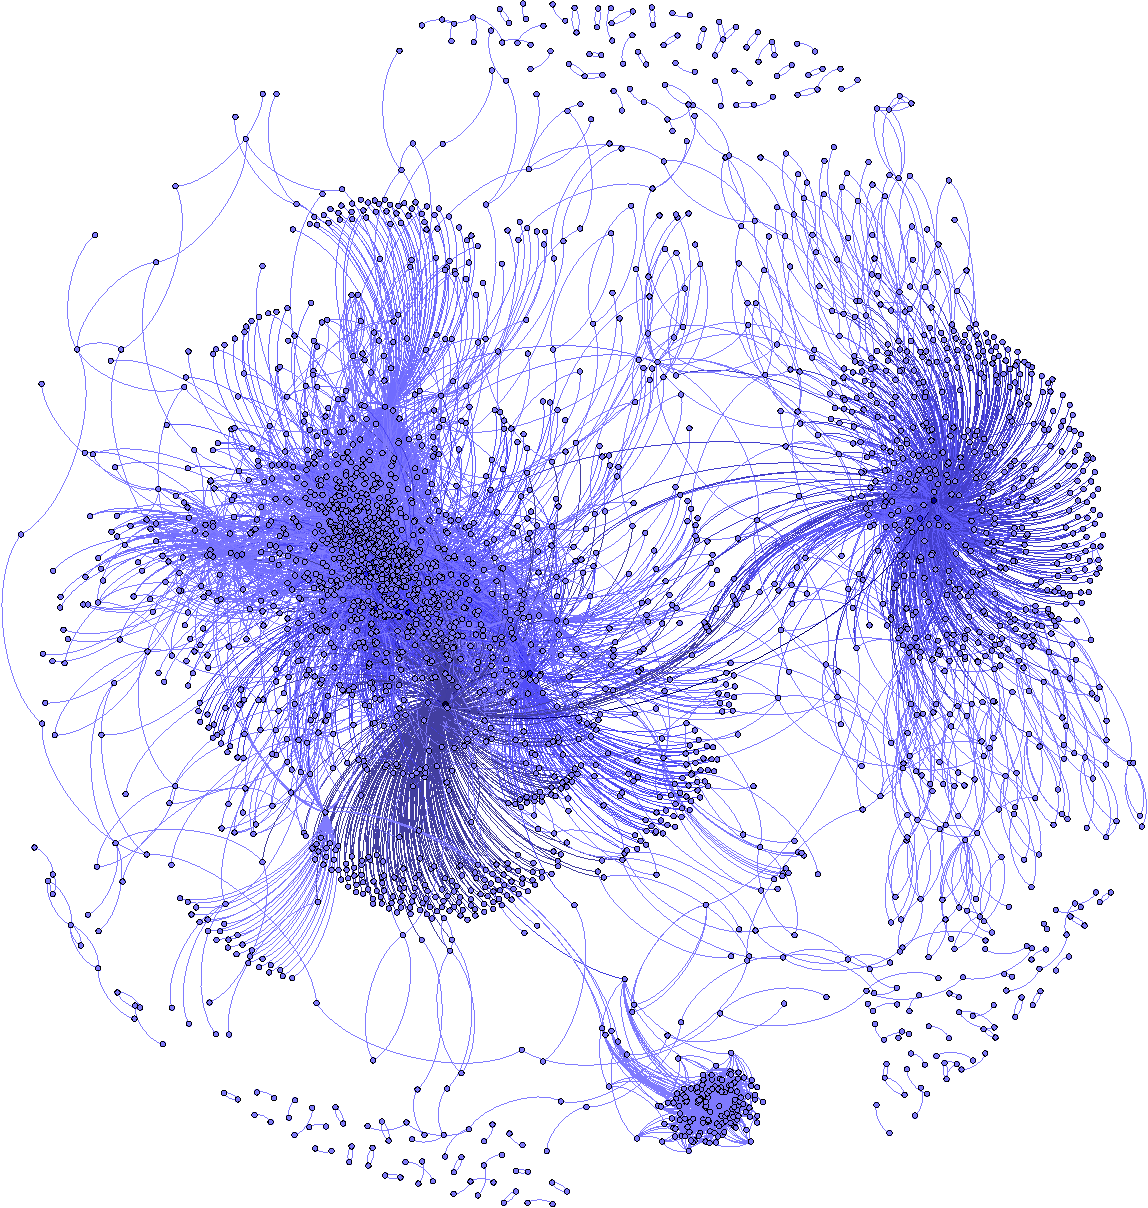
\includegraphics[width=0.5\textwidth]{FIG/graph-crop.pdf}
    \caption{A visualization of the dataset. Each vertex corresponds to a Twitter user and each edge corresponds to a ``following" relationship between two users. A darker node has a higher degree. We can see many disconnected components.}
    \label{fig:twitter}
\end{figure}

\subsection{Dataset}
For analysis, training and testing we use the labelled data collected in the \textsc{Cresci-2018} dataset~\cite{cresci2018fake}. The dataset contains 25,987 user accounts, each of which is assigned a binary label $l \in \{\text{human},\text{bot}\}$ and is the biggest one of its kind that we are aware of. Due to Twitter's developer policy\footnote{https://developer.twitter.com/en/developer-terms/agreement-and-policy.html} which restricts the ways in which user data collected using the Twitter API may be shared, it is difficult to find sizable high-quality datasets. As the rules allow for profile data to be shared online only under specific circumstances and with imposed restrictions, these datasets of fake accounts are typically shared as a set of (user\_id, label) pairs. The associated accounts can then be retrieved again using the Twitter API at a later time. However, as many of the labelled accounts are bots might have been deleted or changed to a ``protected" status which hides most of the profile information from the public. In our case, even though the dataset is relatively recent, only 13,091 of the originally 25,987 labelled accounts were still available (a reduction of about 49.6\%). Of these 6,082 accounts are labelled to be human and 7,009 accounts are labelled as bots (see table~\ref{tab:dataset}).

\begin{table}[t]
\centering
\begin{tabular}{@{}lllllll@{}}
\toprule
       &  & \multicolumn{2}{l}{Ours} &  & \multicolumn{2}{l}{\textsc{Cresci-2018}} \\ \midrule
Humans &  & 6,082       & 46.46\%     &  & 7,479          & 28.78\%         \\
Bots   &  & 7,009       & 54.54\%     &  & 18,508         & 71.22\%         \\ \midrule
\textbf{Total}  &  & \textbf{13,091}      &        &  & \textbf{25,987}         &            \\ \bottomrule
\end{tabular}
\caption{Dataset distribution after retrieving available user profiles using the Twitter API}
\label{tab:dataset}
\end{table}

In addition to the labelled user accounts we have collected all profiles of users followed by or following a user in the dataset. As the Twitter API limits us to a maximum of the first 5,000 users when retrieving these lists we only get those first 5,000 users for users following or followed by more than 5,000 accounts. Including these user profiles we have a total of 4.6 million user profiles. For each user we have the following attributes:

\begin{multicols}{2}
\begin{itemize}
    \item user ID
    \item label
    \item username
    \item screen name
    \item number of “followers” (in-degree)
    \item number of “following” (out-degree)
    \item location
    \item profile URL
    \item profile description
    \item number of times the user is listed
    \item number of favourites
    \item number of status
    \item date created
    \item default profile (boolean)
    \item default profile image (boolean)
    \item list of users followed (up to 5000)
    \item list of followers (up to 5000)
\end{itemize}
\end{multicols}

From this data we can recreate the social graph with distance $d\leq2$ from the users in the \textsc{Cresci-2018} dataset as we have the number of followers and users followed for all users of distance $d=1$ which allows us to simply create ``dummy" nodes without any other attributes in the graph. Unfortunately scraping user profiles of distance $d\geq3$ from the original dataset does not seem feasible for us as this would seem to include a large part of all Twitter accounts and given the Twitter API restrictions might take months. For reference the $90^{th}$-percentile effective diameter of Twitter in 2010 was 4.8~\cite{kwak2010twitter}. A visualization of the graph of all labelled nodes can be seen in figure~\ref{fig:twitter}.

Given this data we perform some basic analysis. When plotting the in-degree-count and out-degree-count graphs we can easily see that bot users tend to have a lower in-degree (less followers) and also a lower out-degree (following less users) than human users. It is worth noting that while the bot accounts seem to mostly follow a power-law, the out-degree distribution for human accounts does not follow a power-law and many nodes in the dataset appear to have a surprisingly high out-degree that may not be perfectly representative of the general user population on Twitter. Further analysis shows that the clustering coefficient of both human and bot accounts appears to be rather low overall which can be explained to the lack of edges and paths that are not included due to the limitations of our crawl of the Twitter network (see figure~\ref{fig:centrality_clustering}). However, we find that the clustering coefficient of human accounts is still slightly higher than that of bot accounts. Regarding the eigenvector centrality we find that human accounts have a slightly higher value too (see also figure~\ref{fig:centrality_clustering}). We believe that these findings may be stronger in a more comprehensive dataset and warrants further investigation in future work.

% GENERAL DEGREE DISTRIBUTION
\begin{figure}[t!]
    \centering
    \begin{subfigure}[t]{0.5\textwidth}
        \centering
        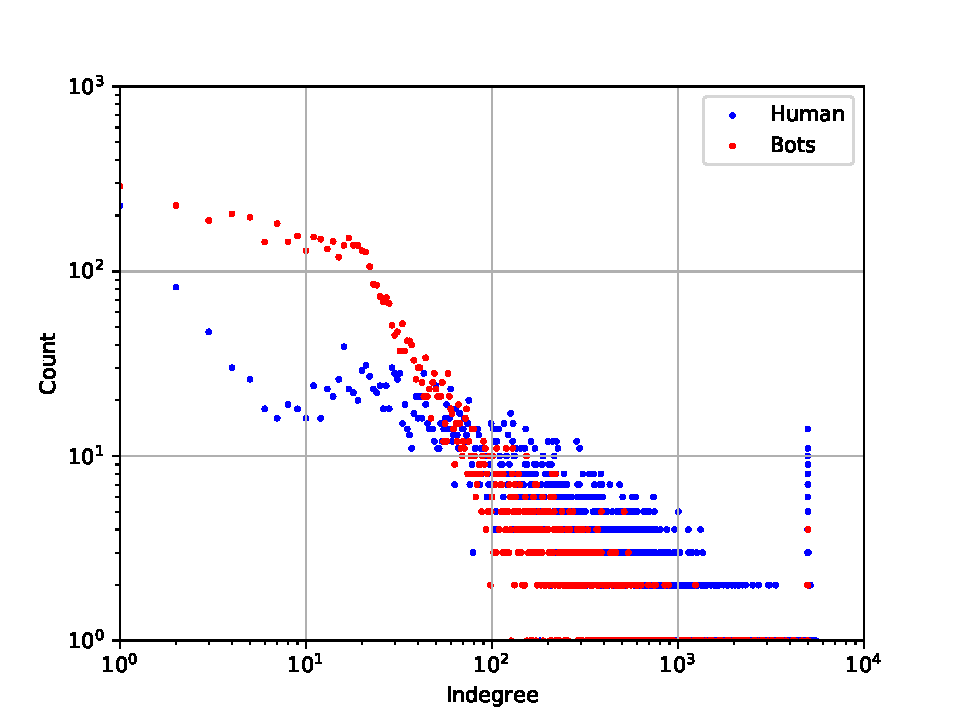
\includegraphics[width=\textwidth]{FIG/indegrees.pdf}
        \caption{In-degree-count graph}
    \end{subfigure}%
    ~
    \begin{subfigure}[t]{0.5\textwidth}
        \centering
        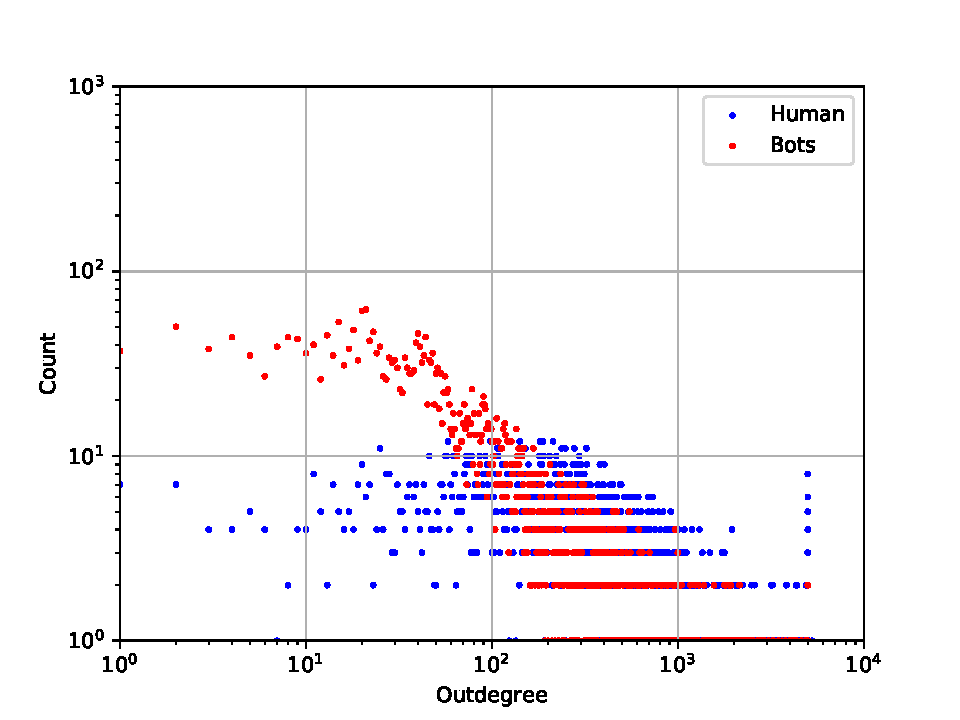
\includegraphics[width=\textwidth]{FIG/outdegrees.pdf}
        \caption{Out-degree-count graph}
    \end{subfigure}
    \caption{Degree-count graphs for human and bot accounts}
    \label{fig:degrees}
\end{figure}

% CENTRALITY AND CLUSTERING COEFFICIENT
\begin{figure}[t!]
    \centering
    \begin{subfigure}[t]{0.5\textwidth}
        \centering
        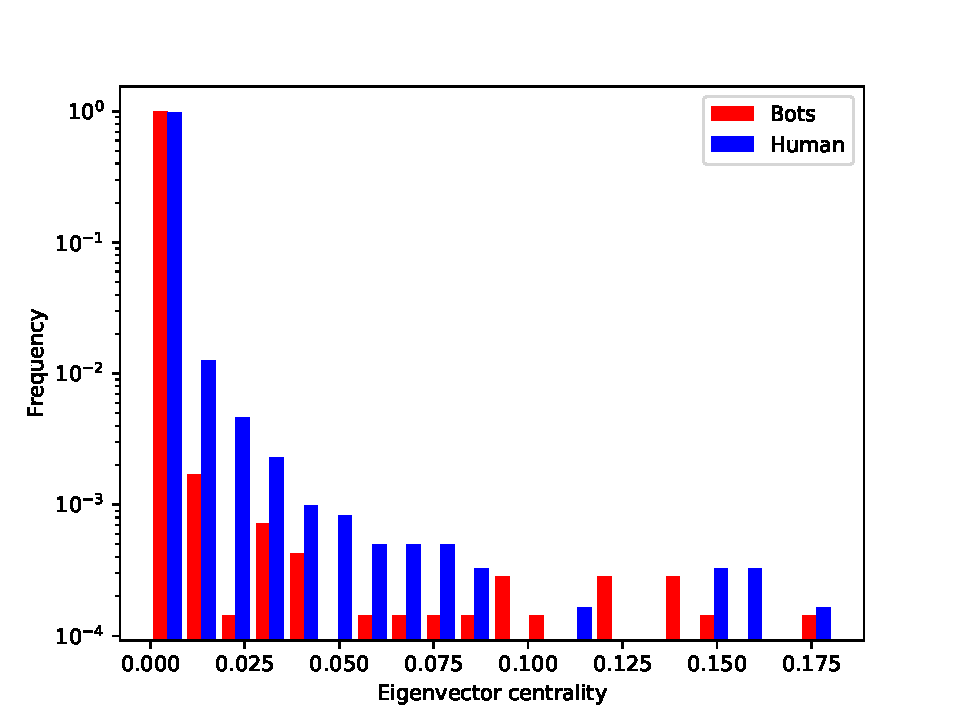
\includegraphics[width=\textwidth]{FIG/centrality.pdf}
        \caption{Eigenvector centrality-frequency graph}
    \end{subfigure}%
    ~
    \begin{subfigure}[t]{0.5\textwidth}
        \centering
        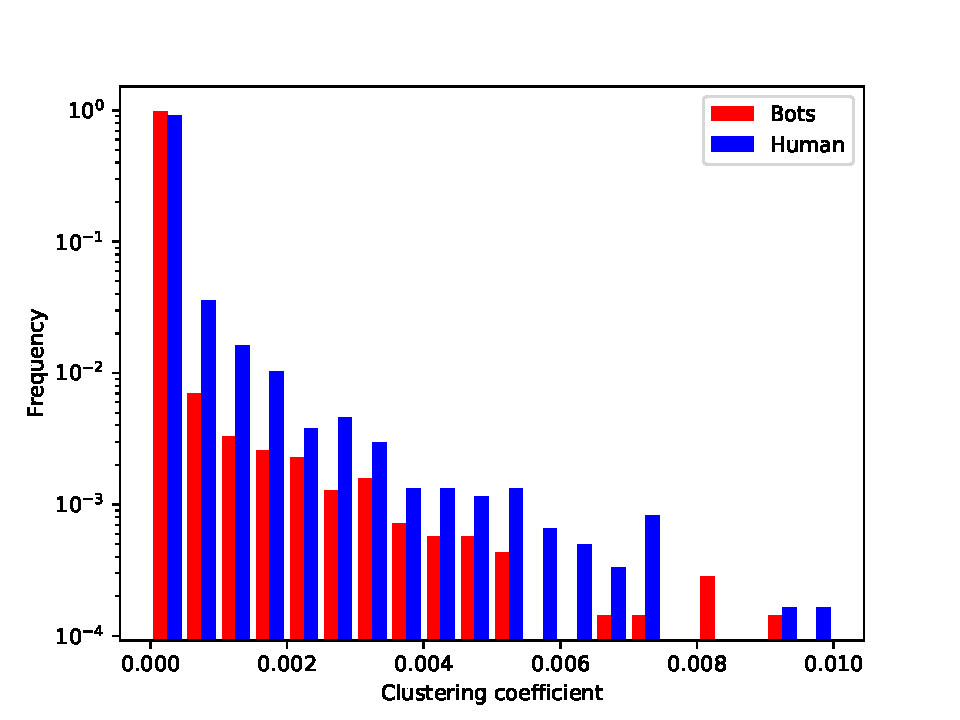
\includegraphics[width=\textwidth]{FIG/coefficient.pdf}
        \caption{Clustering coefficient-frequency graph}
    \end{subfigure}
    \caption{We compare the eigenvector centrality and clustering coefficient distributions among human and bot accounts.}
    \label{fig:centrality_clustering}
\end{figure}


\subsection{Neighborhood-based classification}
\label{sec:approach}

We introduce a novel graph topology and neighborhood-based approach to bot detection. Human and bot accounts typically differ in the way they use Twitter and as a result their structure in the social graph, or their ego graph, is typically different. Instead of classifying a node in the graph just by its immediate features (such as follower count, number of tweets, default profile image etc.) we propose to utilize the graph structure and the features of neighboring nodes in bot classification. We introduce an additional set of features computed as an aggregate over the entire set of predecessors and/or successors. 

% REPUTATION
\begin{figure}[t!]
    \centering
    \begin{subfigure}[t]{0.5\textwidth}
        \centering
        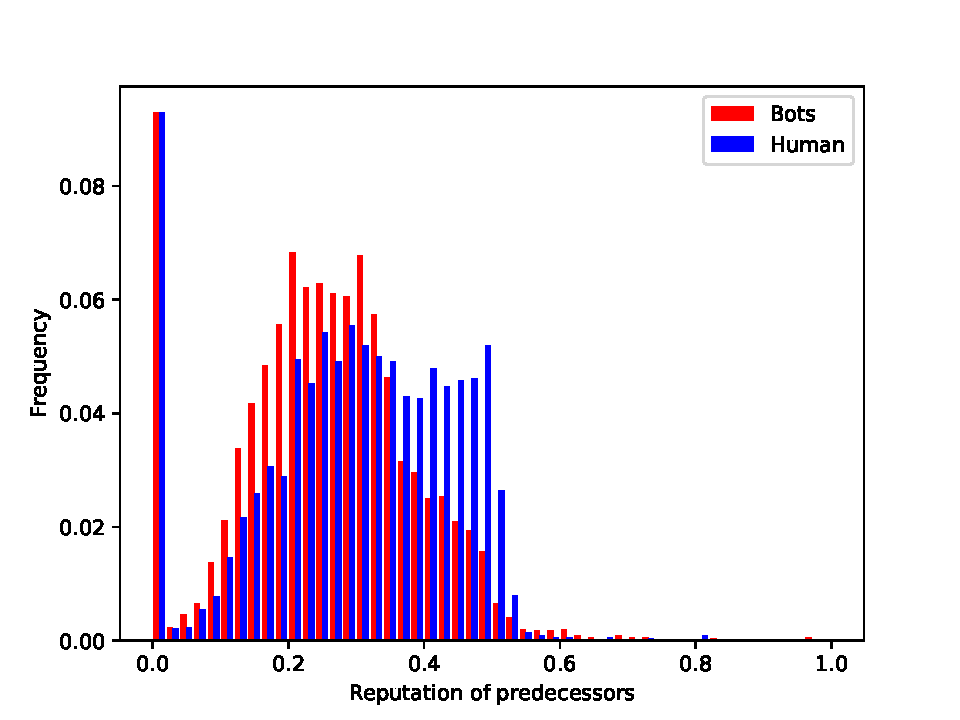
\includegraphics[width=\textwidth]{FIG/reputation_pre.pdf}
        \caption{Aggregated reputation of predecessors}
    \end{subfigure}%
    ~ 
    \begin{subfigure}[t]{0.5\textwidth}
        \centering
        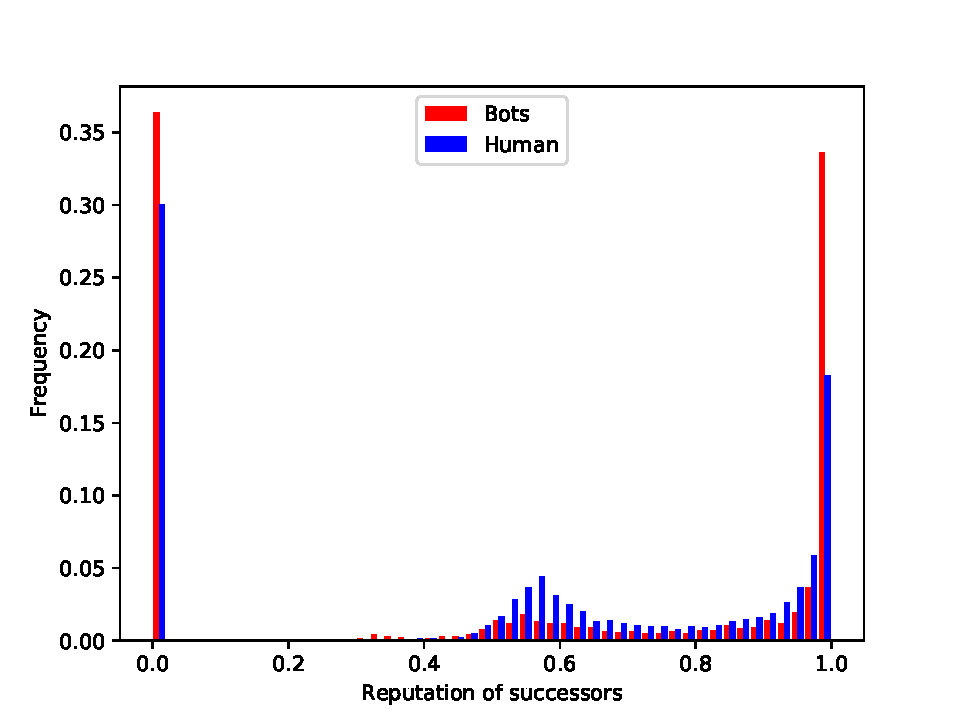
\includegraphics[width=\textwidth]{FIG/reputation_succ.pdf}
        \caption{Aggregated reputation of successors}
    \end{subfigure}
    \caption{We compare the aggregated reputation of users following (predecessors) or followed by (successors) a given user over all human and bot accounts.}
    \label{fig:reputation}
\end{figure}

We will first compute such aggregate features for the dataset using the social graph. In addition to the features scraped using the Twitter API, we computed and evaluated the following features during our analysis. An aggregate of a  feature for a user's neighborhood (a \emph{neighborhood feature}) can be computed by taking the median value across all predecessors or successors (see figure~\ref{fig:reputation}). An aggregate of this measure can be computed across all predecessors/successors by taking the median (see figure~\ref{fig:reputation}).

% DEGREE PREDECESSORS
\begin{figure}[t!]
    \centering
    \begin{subfigure}[t]{0.5\textwidth}
        \centering
        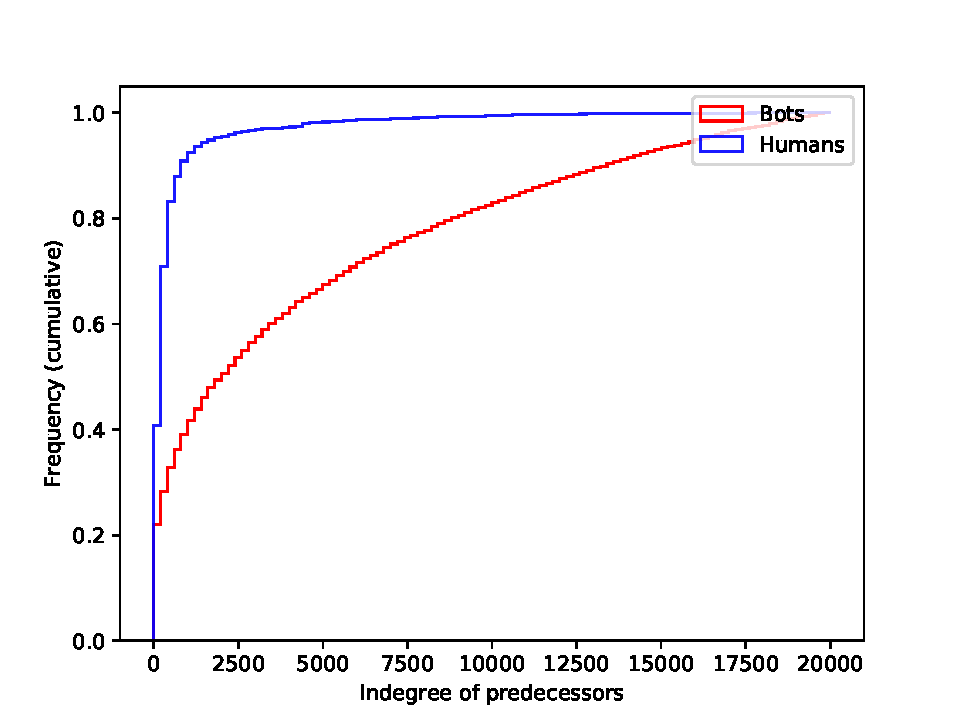
\includegraphics[width=\textwidth]{FIG/indegree_pre.pdf}
        \caption{in-degree}
    \end{subfigure}%
    ~ 
    \begin{subfigure}[t]{0.5\textwidth}
        \centering
        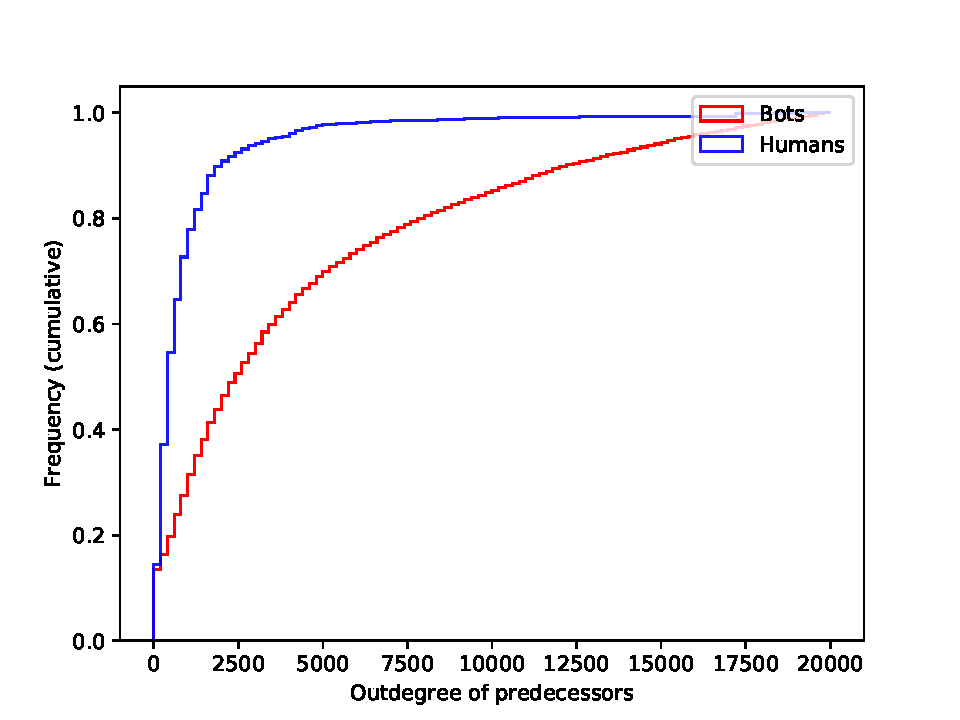
\includegraphics[width=\textwidth]{FIG/outdegree_pre.pdf}
        \caption{out-degree}
    \end{subfigure}
    \caption{Cumulative aggregated degree distribution of predecessor nodes, i.e. median degree of users following by a given user over all bot and human accounts.}
    \label{fig:cum_degrees_predecessors}
\end{figure}

% DEGREE SUCCESSORS
\begin{figure}[t!]
    \centering
    \begin{subfigure}[t]{0.5\textwidth}
        \centering
        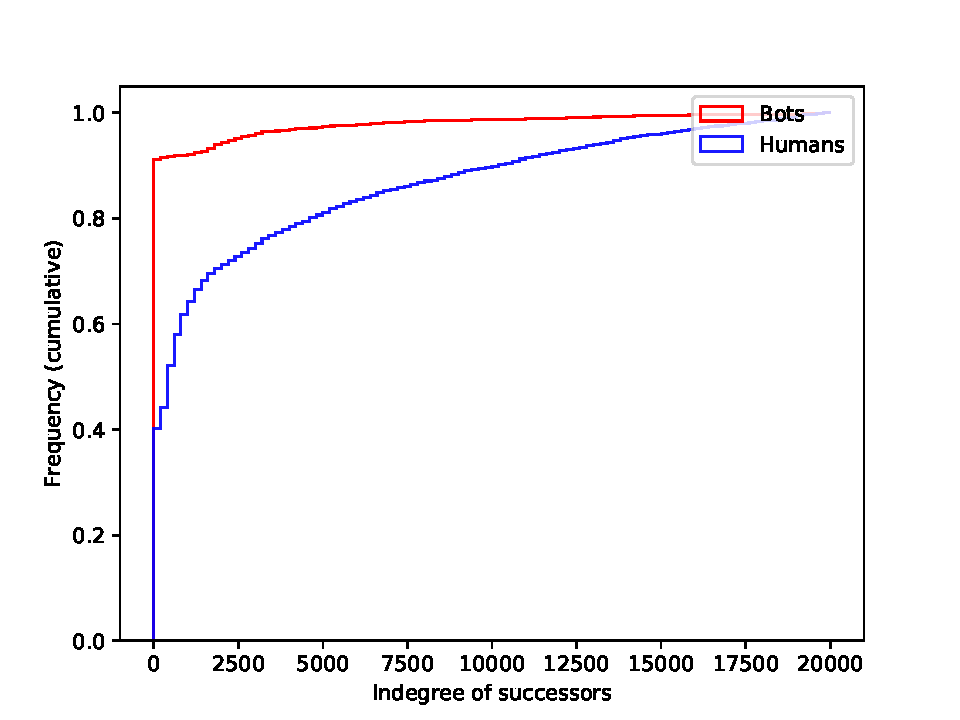
\includegraphics[width=\textwidth]{FIG/indegree_succ.pdf}
        \caption{in-degree}
    \end{subfigure}%
    ~ 
    \begin{subfigure}[t]{0.5\textwidth}
        \centering
        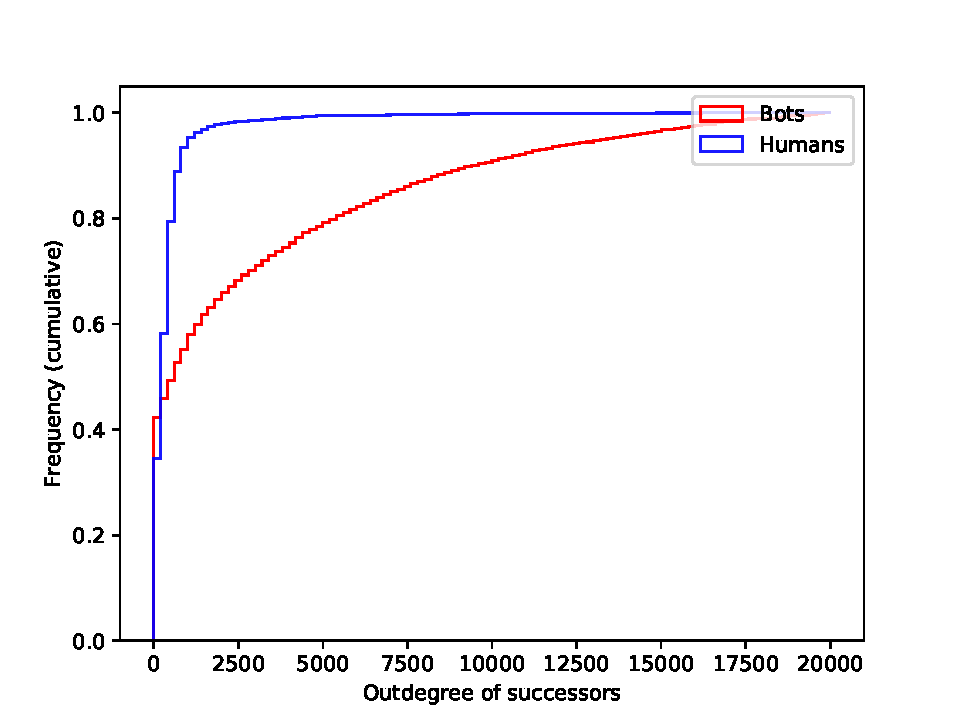
\includegraphics[width=\textwidth]{FIG/outdegree_succ.pdf}
        \caption{out-degree}
    \end{subfigure}
    \caption{Cumulative aggregated degree distribution of successors nodes, i.e. median degree of users followed by a given user over all bot and human accounts.}
    \label{fig:cum_degrees_successors}
\end{figure}

\paragraph{Reputation.} A user's reputation is often measured as the following/follower ratio. We define the reputation $r$ of a user $u$ by
\begin{align*}
    r_u = \frac{ |u_\text{followers}| }{ |u_\text{followers}| + |u_\text{following}|}.
\end{align*}

\paragraph{Median indegree.} We compute median indegree of successors and the median indegree of predecessors. Intuitively, we believe humans tend to follow more high-indegree users (i.e.) news sites, celebrities, while being followed by other low-indegree users.

\paragraph{Median outdegree.} We compute median outdegree of successors and the median outdegree of predecessors. The intuition is that bots may be more likely to be followed by bots or users that follow a large amount of people.

\paragraph{Median reputation.} The above measure of reputation, that is $r_u = \frac{ |u_\text{followers}| }{ |u_\text{followers}| + |u_\text{following}|}$, aggregated for predecessors and successors in the social graph each. Intuitively, real accounts 

\paragraph{Median status count.} Median of status updates for predecessors and successors in the social graph.

\paragraph{Median favourites count.} Median number of favourites or likes by a user's predecessors and successors.

\paragraph{Median listed count.} Median number of times a user's predecessors and successors appear in other users lists on Twitter.

\paragraph{Median account age.} The median account age of predecessors and successors in the social graph. Intuitively, older accounts tend to be more likely to be real users whereas recently created accounts may be bot accounts.

\paragraph{Number of egograph edges.} The total number of edges in a user's egograph. Used to measure how connected the egograph is.

\paragraph{Number of egograph nodes.} The total number of nodes in a user's egograph. Used to measure how connected a user is in the social graph.

\paragraph{Density.} The density of a user's egograph. A graph's density describes the number of edges in relation to the number of nodes. A complete graph has density 1 while a graph with an empty set of edges has density 0. For $n$ nodes and $m$ edges, it is computed as
\begin{align*}
    d = \frac{m}{n(n-1)}.
\end{align*}

\paragraph{Reciprocity.} We measure reciprocity in each user's egograph by computing the ratio of edges that are reciprocated (i.e. that point in both directions) to the total number of edges in the egograph. That is
\begin{align*}
   \mathrm{rec}_G = \frac{|\{(u,v) \ | \ (u,v) \in E \wedge (v,u) \in E \}|}{|\{ (u,v) \ | \ (u,v) \in E \}|}
\end{align*}

\paragraph{Assortativity.} A graph's assortativity measures the similarity of nodes in a graph given a certain attribute. In this case we choose to use ( indegree assortativity (i.e. follower assortativity) to describe how similar a user's egograph is in terms of indegrees.


\bigskip

We find that overall successors appear to have a higher reputation than predecessors. This observation makes sense as many users follow high-degree, high-reputation nodes such as news sources, which in turn are not likely to be following them back. We can also make the observation that human nodes tend to have more reputable predecessors. Additionally, the distribution of reputation of successors is extremely skewed to both extremes for bots which indicates most of them they either follow very reputable nodes or nodes with very low reputation. While the distribution is also extreme for humans, it is not skewed quite as strongly and has many more nodes with a reputation $0.1 < r < 0.9$.

When looking at the cumulative degree distribution among predecessors (figure~\ref{fig:cum_degrees_predecessors}) and successors (figure~\ref{fig:cum_degrees_successors}) we find that many bot accounts in the dataset have predecessors with very high in-degree and out-degree whereas most genuine accounts seem to have lower predecessor degree distributions. For successors however, human accounts tend to have successors with a higher in-degree and lower out-degree, which is in line with our observations regarding the reputation and again indicating that human users tend to follow more accounts with many followers such as news accounts or celebrities. 

%\noindent
%\textit{Logistic regression.} Given a set of $m$ trainings samples $S = \{ (x^{(i)}, y^{(i)}) \}_{i=1}^m$ where $x^{(i)}$ responds to the input features and $y^{(i)}$ in $\{ 0,1 \}$ to the labels, we can model logistic regression as
%$$
%p(y=1|x,\theta) = \frac{1}{1+\text{exp}(-\theta^T x)}
%$$
%with model parameters $\theta$.
